%% why Morita equivalence is important to me

%% -- spirit of Putnam, but without falling into ``everything goes''

%% a false dilemma (forced to the sides of the spectrum, see old
%% Rutgers talk)

\documentclass[fleqn]{beamer}
\usetheme{metropolis}
\usepackage[utf8]{inputenc}
\usepackage[T1]{fontenc}
\usepackage{amsmath, amssymb}
\usepackage{graphicx}
\usepackage{hyperref}
\usepackage{amsfonts}

\usepackage{tikz}
\usetikzlibrary{arrows.meta,decorations.markings,positioning,cd,calc,fit,shapes.multipart,decorations.pathmorphing}

\title{Equivalence: State of Play}
\subtitle{}
\author{Hans Halvorson}
\institute{Princeton University}
\date{April 4, 2025}

%% maybe Visser on 2-cat of theories

%% Sider's worries about our approach

\usepackage[style=authoryear, backend=biber, natbib=true, doi=true]{biblatex} % Chicago style with Biber backend
\addbibresource{morita.bib}

\tikzcdset{every label/.append style = {font = \normalsize}}  % or \scriptsize, etc.

\begin{document}

\begin{frame}
  \titlepage
\end{frame}

\begin{frame}{Introduction}

\centering
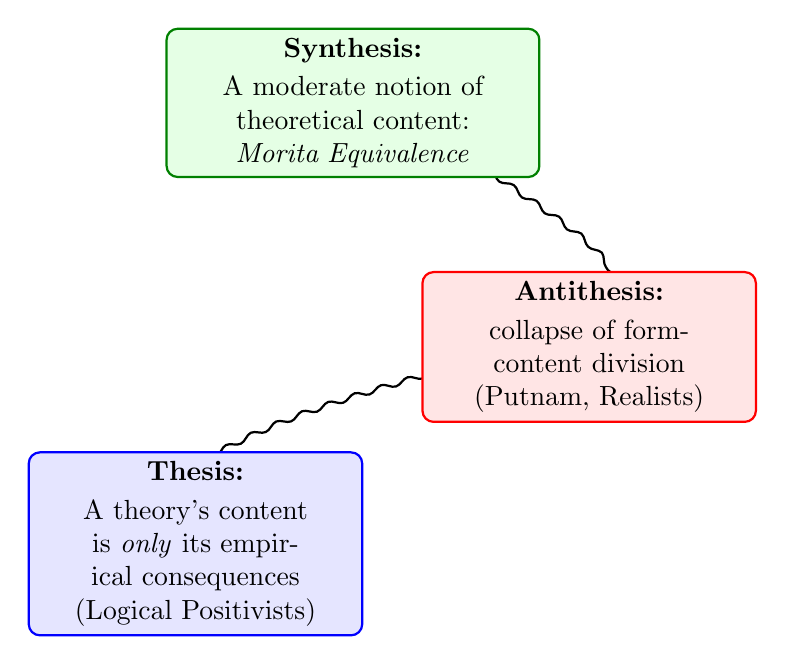
\begin{tikzpicture}[scale=1, every node/.style={align=center}]

\draw[thick,->,decorate,decoration={snake,segment length=10pt,amplitude=1pt,post length=1mm}] 
    (-3,-1) to[out=30,in=210] 
    (2,1) to[out=30,in=225] 
    (0,4);

  % Thesis (bottom)
  \node[fill=blue!10,draw=blue,rounded corners,thick,text width=4cm] at (-3,-2) {
    \textbf{Thesis:} \\[2pt]
    A theory's content is \textit{only} its empirical consequences\\
    (Logical Positivists)
  };

  % Antithesis (middle)
  \node[fill=red!10,draw=red,rounded corners,thick,text width=4cm] at (2,0.5) {
    \textbf{Antithesis:} \\[2pt]
    collapse of form-content division\\
    (Putnam, Realists)
  };

  % Synthesis (top)
  \node[fill=green!10,draw=green!50!black,rounded corners,thick,text
  width=4.5cm] at (-1,3.6) {
    \textbf{Synthesis:} \\[2pt]
    A moderate notion of theoretical content:\\
    \textit{Morita Equivalence} };

\end{tikzpicture}


\end{frame}


% Add your content frames here
\begin{frame}{Outline}
  \tableofcontents
\end{frame}

% \begin{frame}{The epistemological question}

%   \begin{itemize}
%   \item How fine-grained is theory acceptance (belief)?
%   \item What decisions are we faced with?
%   \item What is the significance of these decisions? %% am also faced
%     %% with decision of what color pen to use, but that seems like a
%     %% decision of another kind
%   \end{itemize}

% \end{frame}

% \begin{frame}{The phenomena of equivalence}

%   \begin{itemize}
%   \item Natural language translation
%   \item Scientific disagreement
%     \begin{itemize}
%     \item Wave- and matrix mechanics
%     \item Lorentz versus Einstein
%     \end{itemize}
%   \end{itemize}



% \end{frame}



\section{Notions of equivalence I}

\begin{frame}{Spectrum of Notions of Equivalence}

\hspace*{-0.5cm}
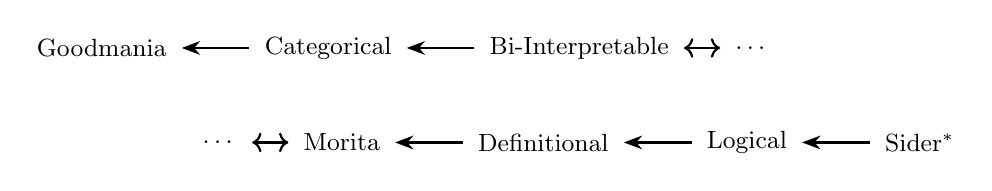
\begin{tikzpicture}[
  node distance=0.8cm and 1.0cm,
  every node/.style={font=\small},
  arrow/.style={-Stealth, thick, shorten >=2pt, shorten <=2pt}, % arrow points in direction of drawing
  doublearrow/.style={<->, thick, shorten >=2pt, shorten <=2pt},
  ]

% Top row (Zeno on the far left)
\node (zeno) at (0,0) {Goodmania};
\node (categorical) [right=of zeno] {Categorical};
\node (biinterp) [right=of categorical] {Bi-Interpretable};
\node (dots1) [right=0.6cm of biinterp] {\ldots};

% Bottom row (Heraclitus on the far right)
\node (dots2) at ($(zeno) + (1.5cm,-1.2cm)$) {\ldots};
\node (morita) [right=0.6cm of dots2] {Morita};
\node (cde) [right=of morita] {Definitional};
\node (logical) [right=of cde] {Logical};
\node (heraclitus) [right=of logical] {Sider$^*$};

% Top row arrows (←)
\draw[arrow] (categorical) -- (zeno);
\draw[arrow] (biinterp) -- (categorical);
\draw[doublearrow] (dots1) -- (biinterp);

% Bottom row arrows (←)
\draw[arrow] (heraclitus) -- (logical);
\draw[arrow] (logical) -- (cde);
\draw[arrow] (cde) -- (morita);
\draw[doublearrow] (dots2) -- (morita);

\end{tikzpicture}

\end{frame}

\begin{frame}{Logical equivalence}

  \begin{itemize}
  \item \textbf{Defn.} $(T_1,\Sigma _1)$ is \textbf{logically
      equivalent} to $(T_2,\Sigma _2)$ just in case
    $\Sigma _1=\Sigma _2$ and $T_1\vdash\varphi$ iff
    $T_2\vdash\varphi$.
  \item Extremely strict because $T_1$ and $T_2$ must use \textbf{same
      symbols}.
  \item Sameness of symbols is not a clear notion. E.g.\ is ``$p$''
    the same symbol as ``$\mathfrak{p}$''?
  \end{itemize}



\end{frame}

\begin{frame}{Definitional equivalence}

  \textbf{Defn.} $T'$ is a \textbf{definitional extension} of $T$ just
  in case $T'=T\cup \{ \delta _1,\dots ,\delta _n\}$ where each
  $\delta _i$ defines a new (relation, function, constant) symbol.

  \bigskip \textbf{Defn.} $T_1$ and $T_2$ are \textbf{definitionally
    equivalent} just in case they have a common definitional extension
  $T^+$.

  \begin{tikzpicture}[
  node distance=1.5cm and 1.5cm,
  every node/.style={font=\small},
  arrow/.style={->, thick, shorten >=2pt, shorten <=2pt},
  ]

% Nodes
\node (Tplus) at (0,2) {$T^+$};
\node (T1) at (-2,0) {$T_1$};
\node (T2) at (2,0) {$T_2$};

% Arrows
\draw[arrow] (T1) -- (Tplus);
\draw[arrow] (T2) -- (Tplus);

\end{tikzpicture}

\end{frame}

\begin{frame}{Definitional Equivalence: Partial Orders with \texorpdfstring{$<$}{<} vs.\ \texorpdfstring{$\leq$}{≤}}

\scriptsize
\begin{center}
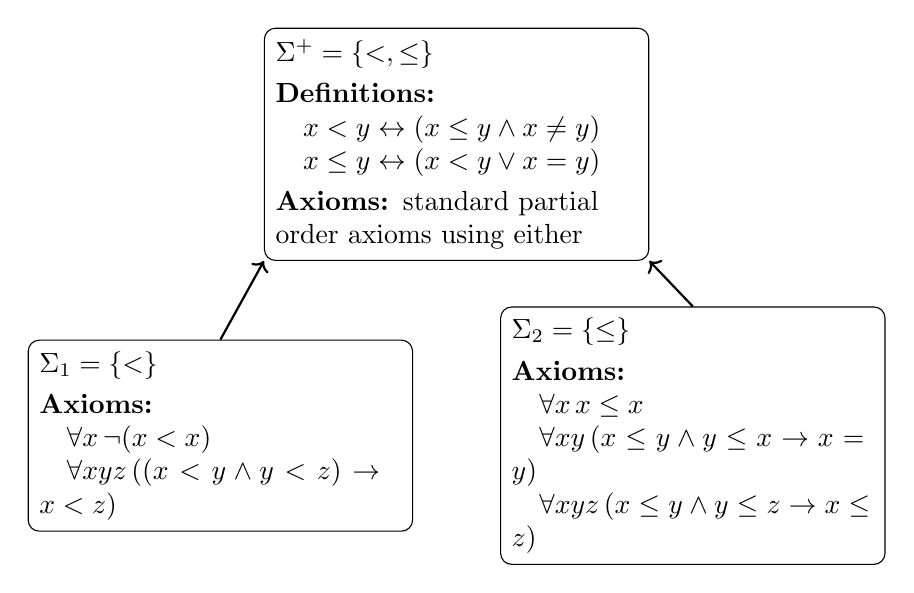
\begin{tikzpicture}[
  every node/.style={align=left},
  box/.style={rectangle, draw, rounded corners, text width=4.6cm, minimum height=2.0cm, inner sep=4pt},
  arrow/.style={->, thick},
  node distance=0.8cm and 1cm
]

% Top node: T^+
\node[box] (Tplus) at (0,3.7) {
  \( \Sigma^+ = \{ <, \leq \} \)\\[0.3em]
  \textbf{Definitions:}\\
  \quad \( x < y \leftrightarrow (x \leq y \land x \neq y)  \)\\
  \quad \( x \leq y \leftrightarrow (x < y \lor x = y) \)\\[0.3em]
  \textbf{Axioms:} standard partial order axioms using either
};

% Bottom left: T1
\node[box] (T1) at (-3,0) {
  \( \Sigma_1 = \{ < \} \)\\[0.3em]
  \textbf{Axioms:}\\
  \quad \( \forall x\, \neg(x < x) \)\\
  \quad \( \forall x y z\, ((x < y \land y < z) \rightarrow x < z) \)
};

% Bottom right: T2
\node[box] (T2) at (3,0) {
  \( \Sigma_2 = \{ \leq \} \)\\[0.3em]
  \textbf{Axioms:}\\
  \quad \( \forall x\, x \leq x \)\\
  \quad \( \forall x y\, (x \leq y \land y \leq x \rightarrow x = y) \)\\
  \quad
  \( \forall x y z\, (x \leq y \land y \leq z \rightarrow x \leq z) \)
};

% Arrows
\draw[arrow] (T1.north) -- (Tplus.south west);
\draw[arrow] (T2.north) -- (Tplus.south east);

\end{tikzpicture}
\end{center}

\end{frame}

\begin{frame}{Morita extensions}
\centering
\begin{tikzpicture}[scale=1, every node/.style={font=\small}]
  % Product (bottom-left)
  \node at (-2,-1) {\textbf{Product}};
  \node (prod) at (-2,-1.75) {$\sigma_0 \times \sigma_1$};
  \node (s0) at (-3,-3) {$\sigma_0$};
  \node (s1) at (-1,-3) {$\sigma_1$};
  \draw[->] (prod) -- (s0);
  \draw[->] (prod) -- (s1);

    % Coproduct (bottom-right)
  \node at (3,-1) {\textbf{Coproduct}};
  \node (s0cop) at (2,-3) {$\sigma_0$};
  \node (s1cop) at (4,-3) {$\sigma_1$};
  \node (cop) at (3,-1.75) {$\sigma_0 \coprod \sigma_1$};
  \draw[->] (s0cop) -- (cop);
  \draw[->] (s1cop) -- (cop);


  % Quotient (top-left)
  \node at (-2,2.5) {\textbf{Quotient}};
  \node (sigma) at (-2,2) {$\sigma$};
  \node (sigmaq) at (-2,1) {$\sigma'$};
  \draw[->] (sigma) -- node[right] {$e$} (sigmaq);

  % Subsort (top-right)
  \node at (3,2.5) {\textbf{Subsort}};
  \node (sigmap) at (3,1) {$\sigma'$};
  \node (sigma2) at (3,2) {$\sigma$};
  \draw[->] (sigmap) -- node[right] {$i$} (sigma2);

\end{tikzpicture}
\end{frame}



\begin{frame}{Morita equivalence}

\centering
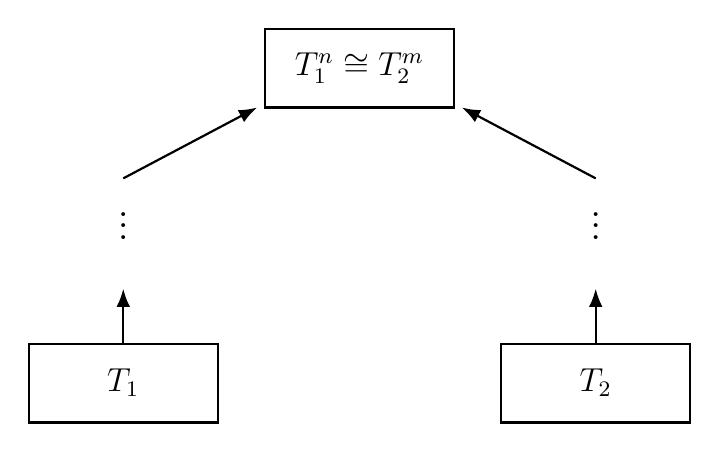
\begin{tikzpicture}[
  theory/.style={rectangle, draw, minimum width=2.4cm, minimum height=1cm, font=\large},
  >=Latex, thick
]

% Base theories
\node[theory] (T1) at (0, 0) {$T_1$};
\node[theory] (T2) at (6, 0) {$T_2$};

% Top node: equivalent theories
\node[theory] (Top) at (3, 4) {$T_1^n \cong T_2^m$};

% Left path: T1 to Top
\draw[->] (T1) -- ++(0,1.2);
\node at ($(T1)+(0,2.1)$) {\Large $\vdots$};
\draw[->] ($(T1)+(0,2.6)$) -- ($(Top)+(-1.3,-0.5)$);

% Right path: T2 to Top
\draw[->] (T2) -- ++(0,1.2);
\node at ($(T2)+(0,2.1)$) {\Large $\vdots$};
\draw[->] ($(T2)+(0,2.6)$) -- ($(Top)+(1.3,-0.5)$);

\end{tikzpicture}
  

\end{frame}


%% here I discuss the geometry construction 

\begin{frame}{Points and lines}

  \hspace*{-1em} 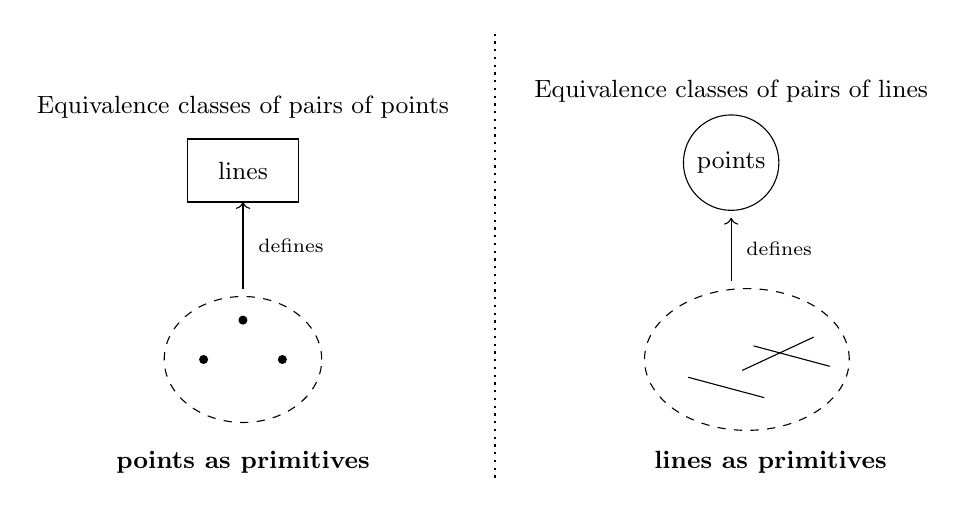
\begin{tikzpicture}[every node/.style={font=\small}, scale=1]

  % Left side: Points primitive

\begin{scope}[shift={(-2,0)}] 
  
\node (p1) at (-3.2,0) [circle,draw,fill=black,inner sep=1pt] {};
\node (p2) at (-2.7,0.5) [circle,draw,fill=black,inner sep=1pt] {};
\node (p3) at (-2.2,0) [circle,draw,fill=black,inner sep=1pt] {};
\draw[dashed] (-2.7,0) ellipse (1.0 and 0.8);

\node at (-2.7,-1.3) {\textbf{points as primitives}};

\draw[->] (-2.7,0.9) -- (-2.7,2) node[midway, right=2pt] {\scriptsize defines};

\node (lineA) at (-2.7,2.4) [rectangle, draw, minimum width=1.4cm, minimum height=0.8cm] {lines};

\node at (-2.7,3.2) {Equivalence classes of pairs of points};

\end{scope}

% Right side: Lines primitive

\begin{scope}[shift={(-1.5,-0.5)}] 

\draw[rotate=25] (3.0,-1) -- +(1.0,0); % Line 1
\draw[rotate=-15] (2.3,0.9) -- +(1.0,0); % Line 2
\draw[rotate=-15] (3.0,1.5) -- +(1.0,0); % Line 3
\draw[dashed] (3.2,0.5) ellipse (1.3 and 0.9);


\node at (3.5,-0.8) {\textbf{lines as primitives}};

\draw[->] (3.0,1.5) -- (3.0,2.3) node[midway, right=2pt] {\scriptsize defines};

\node (pointB) at (3.0,3.0) [circle, draw, minimum size=0.6cm] {points};

\node at (3.0,3.9) {Equivalence classes of pairs of lines};

\end{scope}

% Divider
\draw[dotted, thick] (-1.5,-1.5) -- (-1.5,4.2);

\end{tikzpicture}

\end{frame}

\begin{frame}{Translation Between Theories}

\small

A (generalized) \textbf{translation} from a \( \Sigma \)-theory \( T \)
to a \( \Sigma' \)-theory \( T' \) is based on a \textbf{reconstrual}
\( F: \Sigma \to \Sigma' \), consisting of:

\begin{itemize}
\item A function $F_0: S \to (S')^*$, mapping each sort to a tuple of
  sorts (\textit{dimension function}).
\item A variable mapping
  $x \mapsto \vec{x} = x_1, \dots, x_{d(\sigma)}$, disjoint across
  variables.
\item A domain formula $D_x$ for each variable, natural under
  renaming.
\item A formula $(Fp)(\vec{x}_1, \dots, \vec{x}_n)$ interpreting each
  $\Sigma$-relation symbol $p$ in $\Sigma'$, also natural.
\end{itemize}

This data yields a map \( F\) from \( \Sigma \)-formulas to \( \Sigma' \)-formulas.\\[0.4em]
We say that $F$ is a \textbf{translation} if:
\[ T\vdash \varphi \quad \Rightarrow \quad T' \vdash F(\varphi)
\]

\end{frame}


\begin{frame}{Morita and Translation}

  \begin{itemize}
  \item \textbf{Defn.} An \textbf{equivalence} is a pair of
    translations $F:T\to T'$ and $G:T'\to T$ such that $GF\cong 1_T$
    and $FG\cong 1_{T'}$.
  \item \textbf{Prop.} $T$ and $T'$ are Morita equivalent iff there is
    an equivalence $F:T\to T'$ and $G:T'\to T$.
  \end{itemize}



\end{frame}


\begin{frame}{Examples}

  \begin{tabular}{r|l}
    geometry with points & geometry with lines \\
    \hline nihilism & universalism \\
    \hline two-sorted graphs & one-sorted graphs \\
    \hline ZFC & ETCS \end{tabular}

\end{frame}

\begin{frame}{Counterexamples}

  \begin{itemize}
  \item No two distinct extensions of ZF are
    bi-interpretable. \citep{enayat}
  \end{itemize}

\end{frame}

\section{The semantic turn}


\begin{frame}{Semantic}

  \begin{itemize}
  \item We are considered heterodox for adopting a ``syntactic''
    approach over a ``semantic'' approach. So how to make sense of
    equivalence if a theory is a collection of models?
  \item Model isomorphism criterion: $T_1$ is equivalent to $T_2$ only
    if each model of $T_1$ is isomorphic to some model of $T_2$.
    \begin{itemize}
    \item \citet{north}: Hamiltonian mechanics is not equivalent to
      Lagrangian mechanics because their models are not isomorphic.
    \item The MIC doesn't even follow from definitional equivalence.
    \end{itemize}
  \item Too liberal to require only that there be a bijection between
    classes of models.
  \end{itemize}

\end{frame}


\begin{frame}{From semantics to syntax}

  \begin{itemize}
  \item External structure: e.g.\ arrows between models, nearness
    relations between models
  \item Internal structure: each model of $T_2$ can be ``constructed
    from'' some model of $T_1$.
  \end{itemize}


\end{frame}





\section{Category theory crash course}

\begin{frame}{Categories}

  \centering

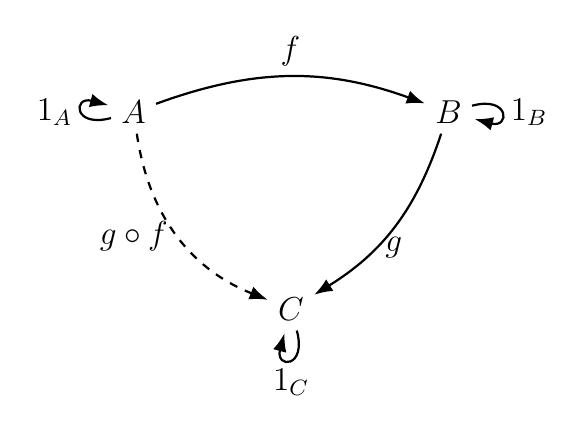
\begin{tikzpicture}[
  every node/.style={font=\large},
  >=Latex, thick
]

% Nodes (objects)
\node (A) at (0,0) {$A$};
\node (B) at (4,0) {$B$};
\node (C) at (2,-2.5) {$C$};

% Arrows (morphisms)
\draw[->] (A) to[bend left=20] node[above] {$f$} (B);
\draw[->] (B) to[bend left=20] node[below] {$g$} (C);
\draw[->, dashed] (A) to[bend right=30] node[left] {$g \circ f$} (C);

% Identity arrows (loops)
\draw[->] (A) edge[loop left] node[left] {$1_A$} (A);
\draw[->] (B) edge[loop right] node[right] {$1_B$} (B);
\draw[->] (C) edge[loop below] node[below] {$1_C$} (C);

\end{tikzpicture}

\end{frame}

\begin{frame}{Functors}

  \centering

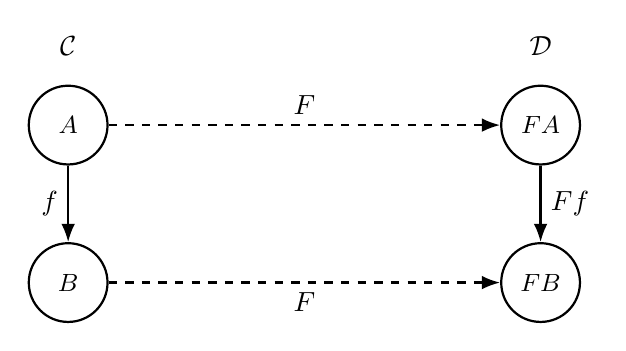
\begin{tikzpicture}[
  object/.style={circle, draw, minimum size=1cm, font=\small},
  ->, >=Latex, thick
]

% Nodes in category C
\node[object] (A) at (0,2) {$A$};
\node[object] (B) at (0,0) {$B$};
\draw[->] (A) to node[left] {$f$} (B);
\node at (0,3) {$\mathcal{C}$};

% Nodes in category D
\node[object] (FA) at (6,2) {$FA$};
\node[object] (FB) at (6,0) {$FB$};
\draw[->] (FA) to node[right] {$Ff$} (FB);
\node at (6,3) {$\mathcal{D}$};

% Dashed arrows indicating functorial action
\draw[->, dashed] (A) -- node[above] {$F$} (FA);
\draw[->, dashed] (B) -- node[below] {$F$} (FB);

\end{tikzpicture}  

\end{frame}

\begin{frame}[fragile]{Natural transformations}

  \centering

\[
\begin{tikzcd}[row sep=2.5em, column sep=3.5em]
  FA \arrow[r, "Ff"] \arrow[d, "\alpha_A"'] & FB \arrow[d, "\alpha_B"] \\
  GA \arrow[r, "Gf"'] & GB
\end{tikzcd}
\]

\end{frame}

\begin{frame}[fragile]{2-categories}

\[
\begin{tikzcd}[column sep=3cm]
  T_1 \arrow[r, bend left=50, "f"{name=U}] 
      \arrow[r, bend right=50, "g"{name=D, swap}] & T_2
  \arrow[
    Rightarrow, 
    from=U, to=D, 
    shorten <=3pt, shorten >=3pt,
    "\chi"'{pos=0.5, xshift=15pt}
  ]
\end{tikzcd}
\]  

\end{frame}

\begin{frame}{Categories of models}

  \begin{itemize}
  \item Each theory $T$ gives rise to a category $\mathrm{Mod}(T)$ of
    models.
  \item If $F:T\to T'$ is a translation then there is a functor
    $F^*:\mathrm{Mod}(T')\to \mathrm{Mod}(T)$.
  \item \textbf{Prop.} If $(F,G)$ is an equivalence of $T$ and $T'$,
    then $(F^*,G^*)$ is an equivalence of $\mathrm{Mod}(T)$ and
    $\mathrm{Mod}(T')$.
  \item It does not follow that if $\mathrm{Mod}(T)$ and
    $\mathrm{Mod}(T')$ are equivalent, then $T$ and $T'$ are
    equivalent.
  \end{itemize}

\end{frame}


\section{Notions of equivalence II}


\begin{frame}{Categorical equivalence}

  \begin{itemize}
  \item \textbf{Defn.} $T$ and $T'$ are \textbf{categorically
      equivalent} just in case $\mathrm{Mod}(T)$ and
    $\mathrm{Mod}(T')$ are equivalent categories.
  \item Pro: Applies even to theories that don't have a first-order
    formulation
  \item Con: The category of a theory's models might omit some of the
    important information about what the theory says.
  \end{itemize}  

\end{frame}

\begin{frame}{Examples}

  \begin{tabular}{r|l}
    Stone spaces & Boolean algebras \\
    \hline Coherent spaces & Rings \\ 
    \hline Relativistic spacetimes & Einstein algebras \\
    \hline Lagrangian mechanics & Hamiltonian mechanics \end{tabular}

\end{frame}


\begin{frame}{Spectrum of Notions of Equivalence}

\hspace*{-0.75cm}
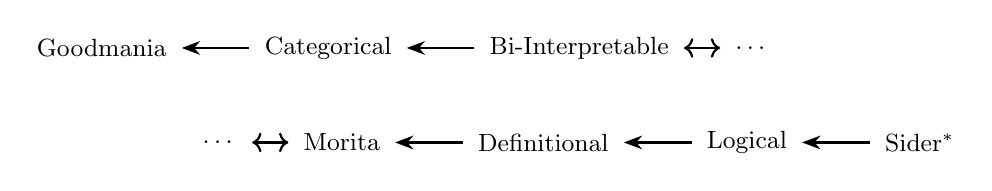
\begin{tikzpicture}[
  node distance=0.8cm and 1.0cm,
  every node/.style={font=\small},
  arrow/.style={-Stealth, thick, shorten >=2pt, shorten <=2pt}, % arrow points in direction of drawing
  doublearrow/.style={<->, thick, shorten >=2pt, shorten <=2pt},
  ]

% Top row (Zeno on the far left)
\node (zeno) at (0,0) {Goodmania};
\node (categorical) [right=of zeno] {Categorical};
\node (biinterp) [right=of categorical] {Bi-Interpretable};
\node (dots1) [right=0.6cm of biinterp] {\ldots};

% Bottom row (Heraclitus on the far right)
\node (dots2) at ($(zeno) + (1.5cm,-1.2cm)$) {\ldots};
\node (morita) [right=0.6cm of dots2] {Morita};
\node (cde) [right=of morita] {Definitional};
\node (logical) [right=of cde] {Logical};
\node (heraclitus) [right=of logical] {Sider$^*$};

% Top row arrows (←)
\draw[arrow] (categorical) -- (zeno);
\draw[arrow] (biinterp) -- (categorical);
\draw[doublearrow] (dots1) -- (biinterp);

% Bottom row arrows (←)
\draw[arrow] (heraclitus) -- (logical);
\draw[arrow] (logical) -- (cde);
\draw[arrow] (cde) -- (morita);
\draw[doublearrow] (dots2) -- (morita);

\end{tikzpicture}

\end{frame}

\begin{frame}{What's the point of talking about equivalence?}

  \begin{itemize}
  \item Simple analogy to ``baby logic''
  \item Rain on metaphysicians' parade?
  \end{itemize}  

\end{frame}




\section{Objections and replies}


%% Teitel, Coffey, Butterfield, Sklar

\begin{frame}{Objection: Equivalence is not a purely formal notion}

  ``One thing we can be sure of. Whatever this structural
  `isomorphism' is to be, it cannot be a purely formal notion. It
  cannot be, that is, an interrelationship which can be determined to
  hold solely on the basis of the logical form of the theories in
  question.'' \citep[p 93]{sklar}

  See: \cite{coffey,teitel,butterfield}
  

  %% citations from the above


\end{frame}

\begin{frame}{Reply}

  \begin{itemize}
  \item Form versus content: What belongs to the content of a theory
    can (always? sometimes?) be represented formally.
  \end{itemize}
  


\end{frame}

%% Sider

\begin{frame}{Quotienting}

  ``According to one alternative --- the second `extreme' approach to
  equivalence I want to discuss --- we can say that theories are
  equivalent without saying why they are equivalent in terms of
  fundamentality and underlying third languages.'' \citep[p
  191]{sider}

\end{frame}


\begin{frame}{Quotienting -- Reply}

  \begin{itemize}
  \item It's a straw person to say that there is no ``reason'' for
    saying that $T$ and $T'$ are equivalent. The existence of a
    translation scheme is a reason!
  \end{itemize}

\end{frame}

%% Calosi - what is Calosi's objection?

\begin{frame}{Blindness}

  \begin{itemize}
  \item \textbf{Objection (Babic and Calosi):} Morita equivalence is
    blind to what gets constructed out of what.
  \item \textbf{Reply:} Granted, there still can be reason to prefer
    one formulation of two Morita equivalent theories.
  \item \textbf{Reply:} Some commitments are shown, and some are
    said. If we say the construction commitment, then the theories are
    not Morita equivalent.
  \end{itemize}


\end{frame}

\begin{frame}{Defending metaphysics}

  \begin{itemize}
  \item \textbf{Objection:} Morita equivalence is part of a sinister
    plot against metaphysics.
  \item \textbf{Reply:} ME may not be consistent with, say, strong
    views about grounding, but ME is not intrinsically
    anti-realist. The permitted definition procedures call for
    metaphysical interpretation.
  \end{itemize}
  
\end{frame}



\section{Open questions}

\begin{frame}{Open questions and projects}

  \begin{itemize}
  \item Is mereological nihilism equivalent to mereological
    universalism (when there are no restrictions on domain size)?
  \item Under what conditions are 4-dimensionalist theories equivalent
    to 3-dimensionalist theories?
  \item Are elementary elliptic and Euclidean geometry equivalent?
    \citep[see][]{glymour}
  \item Notions of equivalence with weaker background assumptions
    \begin{itemize}
    \item Intuitionistic logic and modal S4
    \item Second order logic and many-sorted logic
      \citep[see][]{manzano}
    \end{itemize}
  \end{itemize}


\end{frame}




\section{References}

\nocite{*}


\begin{frame}[allowframebreaks]{References}

\printbibliography[heading=none]

\end{frame}

\end{document}





%%% Local Variables:
%%% mode: latex
%%% TeX-master: t
%%% End:
